\subsubsection{\texttt{RN-1}: aviso a usuarios con navegadores no compatibles con la \textit{File System Access API}}
\label{subsec:rn1}

Tal como se introduce en la \referenciaSeccion{subsec:tecFSA}, la aplicación web hace uso de la \textit{File System Access API}, que es la interfaz que permite que la aplicación web interactúe bidireccionalmente con las carpetas y ficheros del sistema local escogidos por los usuarios. Uno de sus mayores inconvenientes es la divergencia en su compatibilidad, ya que algunos navegadores no implementan esta interfaz, por lo que no permiten esta interacción.

Como consecuencia, algunos de los principales procesos de negocio incorporados en \textit{VSCode4Teaching}, tales como la descarga bajo demanda de los ficheros de las propuestas de los estudiantes por parte de los docentes (\referenciaConTT{subsec:rf4}{RF-4}) o, en el caso de los alumnos, la obtención de los ficheros de sus ejercicios (\referenciaConTT{subsec:rf10}{RF-10}) y la sincronización automática de las modificaciones registradas en los ejercicios durante su realización por parte de los estudiantes (\referenciaConTT{subsec:rf11}{RF-11}), no pueden ser realizados en navegadores no compatibles, mientras que el resto de procesos ya incorporados a la aplicación sí pueden ejecutarse, ya que no dependen del uso de la interfaz para la interacción con el sistema local de ficheros.

Para mejorar la interacción del usuario con la aplicación, este requisito establece la necesidad de informar desde el inicio a los usuarios autenticados acerca de la incompatibilidad de su navegador con la API en caso de acceder mediante, por ejemplo, Firefox o Safari, los navegadores más populares que no soportan esta característica. Con este fin, se introduce en todas las pantallas de la aplicación un aviso, tal como muestra la \referenciaFigura{fig:reqn1-1}, que aconseja el uso de un navegador compatible para poder aprovechar la completitud de las características de la aplicación.

\begin{figure}[ht]
    \centering
    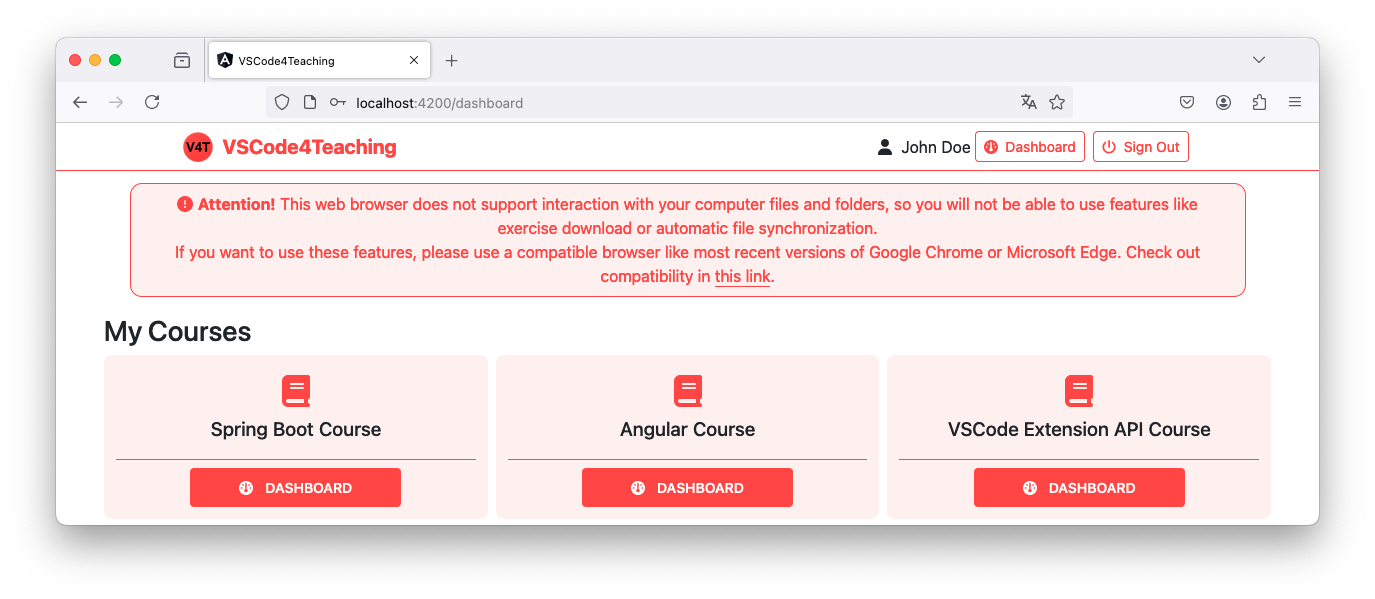
\includegraphics[width=\textwidth]{imagenes/utilizadas/4-3-implementacion/rn1-1.png}
    \caption{\textit{Dashboard} inicial de docentes en Firefox con aviso de incompatibilidad para el uso de la \textit{File System Access API}.}
    \label{fig:reqn1-1}
\end{figure}
